\chapter{Sufficient Statistics and Minimal Representations}
\label{ch:sufficient_stats}

\section{The Quest for the Perfect Representation}

The fundamental objective of representation learning is to distill high-dimensional, complex data into a lower-dimensional, tractable format without losing the salient features necessary for downstream tasks. When we feed an image, a sentence, or a raw audio waveform into a deep neural network, the successive hidden layers transform the data into increasingly abstract representations. But what precisely defines a \emph{good} representation?

From an information-theoretic perspective, a representation is a random variable $Z$ computed from the input data $X$. The defining characteristic of a good representation is that it retains all the necessary information about a target variable $Y$ (such as a class label) while discarding all irrelevant nuances (such as background noise, illumination changes, or font styles). In statistical terms, we want $Z$ to be a \emph{sufficient statistic} for $Y$ with respect to $X$. 

The concept of sufficiency, first introduced by Sir Ronald A. Fisher in 1922, was originally framed in the context of parameter estimation. If one has a set of independent and identically distributed samples drawn from a parameterized distribution, a sufficient statistic is a function of the samples that captures all the information the data provides about the underlying parameter. In the context of deep learning and information theory, we generalize this concept: the "parameter" is replaced by the target variable $Y$. A representation $Z = f_\theta(X)$ is sufficient if observing $Z$ tells us just as much about $Y$ as observing the original, uncompressed data $X$.

However, merely being sufficient is an incredibly weak property on its own. The identity function $Z = X$ is trivially a sufficient statistic, as it retains all information, including the noise. A lossless compression of $X$ is also sufficient, yet neither achieves the goal of abstraction. The true mathematical north star of representation learning is the \emph{minimal sufficient statistic}. 

A minimal sufficient statistic is the ultimate distillation. It is a sufficient statistic that compresses the input data as much as fundamentally possible. It strips away every single bit of entropy in $X$ that does not contribute to predicting $Y$. Geometrically, it groups together all inputs $x \in \mathcal{X}$ that share the exact same posterior distribution $P(Y \mid X=x)$ into a single point in the latent space $\mathcal{Z}$. In doing so, it provides a representation that is not only optimal for the downstream task but also highly invariant to nuisance factors. 

In this chapter, we will formalize the notions of sufficiency and minimality using the language of Shannon information theory. We will prove the Fisher-Neyman Factorization Theorem for random variables, demonstrate how minimal sufficient statistics optimally compress data, and explore how these classical statistical concepts govern the theoretical limits of modern deep neural networks.

\section{Mathematical Foundations of Sufficiency}

We begin by establishing the formal definition of a sufficient statistic using the concept of Markov chains. Let $X \in \mathcal{X}$ be a data random variable, and $Y \in \mathcal{Y}$ be a target random variable, governed by a joint distribution $P_{X,Y}$. A representation $Z \in \mathcal{Z}$ is formed by a potentially stochastic mapping from $X$, meaning that the conditional distribution of $Z$ depends only on $X$. This forms the Markov chain $Y \leftrightarrow X \leftrightarrow Z$.

\begin{definition}[Sufficient Statistic]
A statistic $Z$, derived from $X$ via the Markov chain $Y \leftrightarrow X \leftrightarrow Z$, is said to be \emph{sufficient} for $Y$ if $X$ and $Y$ are conditionally independent given $Z$. That is, the Markov chain $X \leftrightarrow Z \leftrightarrow Y$ also holds, which implies:
\[ P(Y \mid X, Z) = P(Y \mid Z) \]
almost everywhere.
\end{definition}

In the context of deterministic neural networks where $Z = f_\theta(X)$, the variable $Z$ is fully determined by $X$. Consequently, conditioning on both $X$ and $Z$ is equivalent to conditioning on $X$ alone. Thus, the condition for sufficiency simplifies to $P(Y \mid X=x) = P(Y \mid Z=f_\theta(x))$ for all $x$.

\begin{theorem}[Information-Theoretic Sufficiency]
Let $Y \leftrightarrow X \leftrightarrow Z$ form a Markov chain. The statistic $Z$ is sufficient for $Y$ if and only if it preserves the mutual information between $X$ and $Y$, i.e.,
\[ I(Z; Y) = I(X; Y) \]
\end{theorem}
\begin{proof}
By the chain rule for mutual information, we can expand the mutual information between $Y$ and the joint variable $(X, Z)$ in two different ways:
\begin{align*}
I(X, Z; Y) &= I(Z; Y) + I(X; Y \mid Z) \\
I(X, Z; Y) &= I(X; Y) + I(Z; Y \mid X)
\end{align*}
Because $Y \leftrightarrow X \leftrightarrow Z$ is a Markov chain, we have $P(Z \mid X, Y) = P(Z \mid X)$, meaning $Z$ and $Y$ are conditionally independent given $X$. Therefore, $I(Z; Y \mid X) = 0$. Substituting this into the second equation yields:
\[ I(X, Z; Y) = I(X; Y) \]
Equating the two expansions, we get:
\[ I(X; Y) = I(Z; Y) + I(X; Y \mid Z) \]
Since mutual information is non-negative, $I(Z; Y) \le I(X; Y)$, which is the Data Processing Inequality. Equality holds if and only if $I(X; Y \mid Z) = 0$. By definition, $I(X; Y \mid Z) = 0$ is equivalent to the conditional independence $X \perp\!\!\!\perp Y \mid Z$, which is precisely the definition of $Z$ being a sufficient statistic.
\end{proof}

\begin{figure}[htbp]
\centering
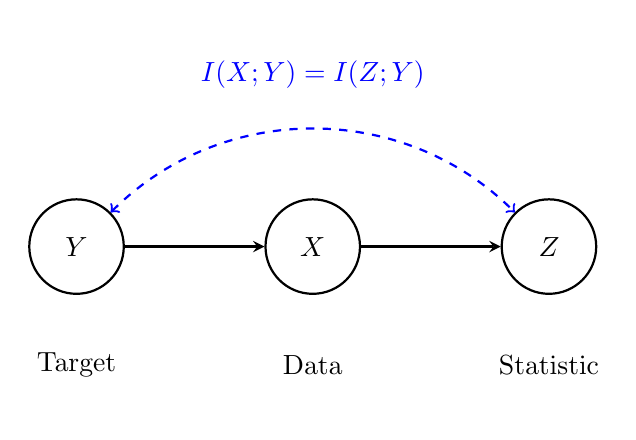
\begin{tikzpicture}[
    scale=1.5,
    every node/.style={circle, draw=black, thick, minimum size=1.2cm, align=center},
    arrow/.style={->, >=stealth, thick}
]
    % Nodes
    \node (Y) at (0,0) {$Y$};
    \node (X) at (2,0) {$X$};
    \node (Z) at (4,0) {$Z$};
    
    % Edges
    \draw[arrow] (Y) -- (X);
    \draw[arrow] (X) -- (Z);
    
    % Labels
    \node[draw=none, rectangle] at (0,-1) {Target};
    \node[draw=none, rectangle] at (2,-1) {Data};
    \node[draw=none, rectangle] at (4,-1) {Statistic};
    
    % Arcs for Markov conditions
    \draw[<->, dashed, thick, blue] (Y) to[out=45, in=135] node[draw=none, rectangle, above, text=blue, yshift=2pt] {$I(X;Y) = I(Z;Y)$} (Z);
\end{tikzpicture}
\caption{The Markov chain $Y \leftrightarrow X \leftrightarrow Z$. A representation $Z$ is a sufficient statistic if it retains all mutual information about $Y$ present in $X$.}
\label{fig:markov_sufficiency}
\end{figure}

A classic algebraic characterization of sufficiency is the Fisher-Neyman Factorization Theorem. While traditionally stated for parameterized distributions $P(X \mid \theta)$, we adapt it here for target random variables $Y$.

\begin{theorem}[Fisher-Neyman Factorization]
\label{thm:fisher_neyman}
A statistic $Z = T(X)$ is sufficient for $Y$ if and only if the joint probability distribution $P(x, y)$ can be factorized as:
\[ P(x, y) = h(x) g(T(x), y) \]
for some non-negative functions $h$ and $g$.
\end{theorem}
\begin{proof}
We provide the proof for discrete random variables. 
First, assume $Z = T(X)$ is a sufficient statistic. The joint distribution can be written as:
\begin{align*}
P(x, y) &= P(x, y, T(x)) \\
&= P(T(x), y) P(x \mid T(x), y)
\end{align*}
By the definition of sufficiency, $X$ and $Y$ are conditionally independent given $T(X)$, meaning $P(x \mid T(x), y) = P(x \mid T(x))$. Thus:
\[ P(x, y) = P(T(x), y) P(x \mid T(x)) \]
This matches the required factorization by setting $g(T(x), y) = P(T(x), y)$ and $h(x) = P(x \mid T(x))$.

Conversely, assume $P(x, y) = h(x) g(T(x), y)$. The marginal distribution of $Y$ given $X=x$ is:
\begin{align*}
P(y \mid x) &= \frac{P(x, y)}{\sum_{y'} P(x, y')} \\
&= \frac{h(x) g(T(x), y)}{\sum_{y'} h(x) g(T(x), y')} \\
&= \frac{g(T(x), y)}{\sum_{y'} g(T(x), y')}
\end{align*}
Notice that the right-hand side depends on $x$ only through the value of $T(x)$. Therefore, for any two inputs $x_1, x_2$ such that $T(x_1) = T(x_2)$, we have $P(y \mid x_1) = P(y \mid x_2)$. This implies $P(Y \mid X, Z) = P(Y \mid Z)$, proving that $Z = T(X)$ is sufficient for $Y$.
\end{proof}

\section{Minimal Sufficient Statistics}

Sufficiency guarantees that no predictive power is lost. However, it does not guarantee that the representation is concise. The input $X$ itself is always trivially sufficient. To achieve true representation learning, we must seek the \emph{minimal} sufficient statistic.

\begin{definition}[Minimal Sufficient Statistic]
A sufficient statistic $Z = T_{min}(X)$ is \emph{minimal} if it can be computed from any other sufficient statistic. Formally, for any sufficient statistic $Z' = T'(X)$, there exists a deterministic function $f$ such that $T_{min}(X) = f(T'(X))$ almost everywhere.
\end{definition}

Geometrically, a statistic $T(X)$ partitions the input space $\mathcal{X}$ into level sets, where all $x$ mapping to the same $z$ belong to the same set. Theorem \ref{thm:fisher_neyman} showed that a sufficient statistic requires the posterior $P(Y \mid X=x)$ to be constant within each level set. A minimal sufficient statistic corresponds to the \emph{coarsest possible partition} of $\mathcal{X}$ that maintains this property. It merges all $x$ that share the exact same posterior distribution into a single equivalence class.

\begin{figure}[htbp]
\centering
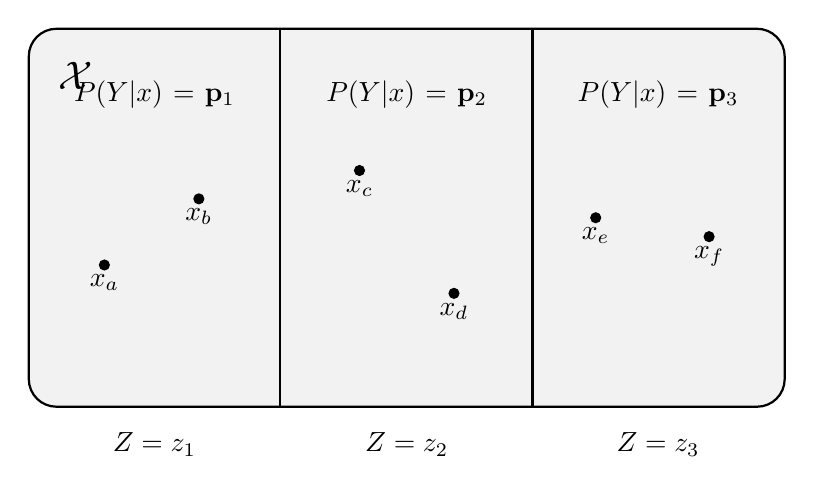
\begin{tikzpicture}[scale=1.2]
    % Draw the X space
    \draw[thick, rounded corners=10pt, fill=gray!10] (0,0) rectangle (8,4);
    \node[draw=none, rectangle] at (0.5, 3.5) {\Large $\mathcal{X}$};
    
    % Draw partitions for Z = T(X)
    \draw[thick] (2.66,0) -- (2.66,4);
    \draw[thick] (5.33,0) -- (5.33,4);
    
    % Z values
    \node[draw=none, rectangle] at (1.33, -0.4) {$Z = z_1$};
    \node[draw=none, rectangle] at (4, -0.4) {$Z = z_2$};
    \node[draw=none, rectangle] at (6.66, -0.4) {$Z = z_3$};
    
    % Posterior distributions
    \node[draw=none, rectangle, text width=2.5cm, align=center] at (1.33, 3.3) {$P(Y|x) = \mathbf{p}_1$};
    \node[draw=none, rectangle, text width=2.5cm, align=center] at (4, 3.3) {$P(Y|x) = \mathbf{p}_2$};
    \node[draw=none, rectangle, text width=2.5cm, align=center] at (6.66, 3.3) {$P(Y|x) = \mathbf{p}_3$};
    
    % Points
    \filldraw (0.8, 1.5) circle (1.5pt) node[anchor=north] {$x_a$};
    \filldraw (1.8, 2.2) circle (1.5pt) node[anchor=north] {$x_b$};
    
    \filldraw (3.5, 2.5) circle (1.5pt) node[anchor=north] {$x_c$};
    \filldraw (4.5, 1.2) circle (1.5pt) node[anchor=north] {$x_d$};
    
    \filldraw (6, 2) circle (1.5pt) node[anchor=north] {$x_e$};
    \filldraw (7.2, 1.8) circle (1.5pt) node[anchor=north] {$x_f$};
    
\end{tikzpicture}
\caption{A minimal sufficient statistic $Z$ partitions the input space $\mathcal{X}$ into the coarsest possible level sets such that the posterior $P(Y \mid X=x)$ remains constant within each subset. Any further compression would merge regions with different posteriors, destroying sufficiency.}
\label{fig:partitions}
\end{figure}

\begin{theorem}[Minimality and Information]
Let $Z = T(X)$ be a sufficient statistic for $Y$. $Z$ is a minimal sufficient statistic if and only if it minimizes the mutual information $I(X; Z)$ among all sufficient statistics.
\end{theorem}
\begin{proof}
Let $Z_{min}$ be a minimal sufficient statistic and $Z$ be any other sufficient statistic. By definition of minimality, there exists a deterministic function $f$ such that $Z_{min} = f(Z)$. This establishes the Markov chain $X \leftrightarrow Z \leftrightarrow Z_{min}$.
Applying the Data Processing Inequality to this chain, we immediately obtain:
\[ I(X; Z_{min}) \le I(X; Z) \]
Since $Z$ was chosen arbitrarily from the set of all sufficient statistics, $Z_{min}$ must attain the global minimum of $I(X; Z)$ within this set. Furthermore, because $Z_{min} = f(Z)$ is a deterministic function, $H(Z_{min} \mid Z) = 0$. The minimization of $I(X; Z)$ subject to the sufficiency constraint $I(Z; Y) = I(X; Y)$ perfectly characterizes the minimal sufficient statistic in an information-theoretic framework.
\end{proof}

\section{Numerical Example: Compressing Binary Sequences}

To ground these concepts, let us construct a concrete numerical example. Suppose our target variable $Y \in \{0, 1\}$ is a binary label drawn with equal probability, $P(Y=1) = P(Y=0) = 0.5$. 
Conditioned on $Y$, our data $X = (X_1, X_2) \in \{0, 1\}^2$ consists of two independent Bernoulli trials. If $Y=1$, the success probability is $0.8$. If $Y=0$, the success probability is $0.2$.

First, we compute the entropy of $Y$:
\[ H(Y) = -0.5 \log_2(0.5) - 0.5 \log_2(0.5) = 1 \text{ bit} \]

Next, we evaluate the joint distribution $P(X, Y)$ and the marginal $P(X)$:
\begin{itemize}
    \item $P(X=(0,0)) = P(Y=1)(0.2)^2 + P(Y=0)(0.8)^2 = 0.5(0.04) + 0.5(0.64) = 0.34$
    \item $P(X=(0,1)) = P(Y=1)(0.8)(0.2) + P(Y=0)(0.2)(0.8) = 0.5(0.16) + 0.5(0.16) = 0.16$
    \item $P(X=(1,0)) = P(Y=1)(0.8)(0.2) + P(Y=0)(0.2)(0.8) = 0.16$
    \item $P(X=(1,1)) = P(Y=1)(0.8)^2 + P(Y=0)(0.2)^2 = 0.5(0.64) + 0.5(0.04) = 0.34$
\end{itemize}

The entropy of the raw data $X$ is:
\begin{align*}
H(X) &= -2(0.34 \log_2 0.34) - 2(0.16 \log_2 0.16) \\
&\approx 2(0.529) + 2(0.423) = 1.904 \text{ bits}
\end{align*}

The conditional entropy $H(Y \mid X)$ requires computing the posterior $P(Y=1 \mid X)$ for each outcome:
\begin{itemize}
    \item $P(Y=1 \mid X=(0,0)) = \frac{0.02}{0.34} = \frac{1}{17}$
    \item $P(Y=1 \mid X=(0,1)) = \frac{0.08}{0.16} = \frac{1}{2}$
    \item $P(Y=1 \mid X=(1,0)) = \frac{0.08}{0.16} = \frac{1}{2}$
    \item $P(Y=1 \mid X=(1,1)) = \frac{0.32}{0.34} = \frac{16}{17}$
\end{itemize}

Computing the weighted sum of binary entropies $H_b(p)$:
\begin{align*}
H(Y \mid X) &= 0.34 H_b\left(\frac{1}{17}\right) + 0.16 H_b\left(\frac{1}{2}\right) + 0.16 H_b\left(\frac{1}{2}\right) + 0.34 H_b\left(\frac{16}{17}\right) \\
&= 0.68 H_b\left(\frac{1}{17}\right) + 0.32(1) \\
&\approx 0.68(0.323) + 0.32 \approx 0.540 \text{ bits}
\end{align*}
The mutual information is $I(X; Y) = H(Y) - H(Y \mid X) = 1 - 0.540 = 0.460$ bits.

Now, define a representation $Z = X_1 + X_2 \in \{0, 1, 2\}$. This statistic merges the states $(0,1)$ and $(1,0)$ into $Z=1$.
Notice that $P(Y=1 \mid X=(0,1)) = P(Y=1 \mid X=(1,0)) = 0.5$. Because the posterior is identical, merging them into a single equivalence class $Z=1$ does not destroy any predictive information.
We can verify this by calculating $I(Z; Y)$:
$P(Z=0) = 0.34$, $P(Z=1) = 0.32$, $P(Z=2) = 0.34$.
The conditional entropies $H(Y \mid Z=z)$ are identically equal to $H(Y \mid X=x)$ for the corresponding $x$.
Thus, $H(Y \mid Z) = 0.540$ bits, and $I(Z; Y) = 0.460$ bits.
Since $I(Z; Y) = I(X; Y)$, $Z$ is indeed a sufficient statistic.

How much did we compress the data?
\begin{align*}
H(Z) &= -0.34 \log_2 0.34 - 0.32 \log_2 0.32 - 0.34 \log_2 0.34 \\
&\approx 0.529 + 0.526 + 0.529 = 1.584 \text{ bits}
\end{align*}
By mapping $X$ to $Z$, we compressed the representation from $1.904$ bits to $1.584$ bits (meaning $I(X; Z) = 1.584$ bits, since $Z$ is deterministic), without losing any of the $0.460$ bits of relevant information about $Y$. Because no further compression is possible without breaking sufficiency, $Z$ is the minimal sufficient statistic for this setup.

\section{Representations in Deep Neural Networks}

In modern deep learning, the mapping $Z = f_\theta(X)$ is parameterized by a neural network, and we typically train the network by minimizing the cross-entropy loss against the true labels $Y$. A natural question arises: does minimizing cross-entropy naturally lead to a sufficient statistic?

Let $q_\phi(Y \mid Z)$ be a parameterized decoder or classification head. The cross-entropy loss over the joint distribution is given by:
\[ \mathcal{L}(\theta, \phi) = \mathbb{E}_{P_{X,Y}} [-\log q_\phi(Y \mid f_\theta(X))] \]

\begin{theorem}[Cross-Entropy and Sufficiency]
If the classifier $q_\phi$ has sufficient capacity to perfectly model the true posterior $P(Y \mid Z)$, then minimizing the cross-entropy loss is equivalent to maximizing the mutual information $I(Z; Y)$. The global minimum is achieved if and only if $Z$ is a sufficient statistic.
\end{theorem}
\begin{proof}
By adding and subtracting $\log P(Y \mid Z)$, the cross-entropy can be rewritten as:
\begin{align*}
\mathcal{L}(\theta, \phi) &= \mathbb{E}_{P_{Z,Y}} [-\log q_\phi(Y \mid Z)] \\
&= \mathbb{E}_{P_{Z,Y}} \left[-\log P(Y \mid Z) + \log \frac{P(Y \mid Z)}{q_\phi(Y \mid Z)} \right] \\
&= H(Y \mid Z) + \mathbb{E}_{P_Z} [D_{\text{KL}}(P(Y \mid Z) \parallel q_\phi(Y \mid Z))]
\end{align*}
Since the Kullback-Leibler divergence is non-negative, the loss is minimized with respect to $\phi$ when $q_\phi(Y \mid Z) = P(Y \mid Z)$ almost everywhere, which zeroes out the KL term.
The remaining term is the conditional entropy $H(Y \mid Z)$. We know that $I(Z; Y) = H(Y) - H(Y \mid Z)$. Since the marginal entropy $H(Y)$ is a constant defined by the dataset, minimizing $H(Y \mid Z)$ via the parameters $\theta$ is mathematically equivalent to maximizing $I(Z; Y)$. 
By the Data Processing Inequality, $I(Z; Y) \le I(X; Y)$. The theoretical minimum of the cross-entropy loss is therefore $H(Y \mid X)$, which is achieved if and only if $I(Z; Y) = I(X; Y)$, i.e., when $Z = f_\theta(X)$ is a sufficient statistic for $Y$.
\end{proof}

While cross-entropy training theoretically encourages the network to extract a sufficient statistic, it provides no explicit incentive for \emph{minimality}. In the absence of an explicit compression penalty, a high-capacity neural network might retain nuisance information, leading to suboptimal generalization. This fundamental limitation sets the stage for the Information Bottleneck Principle.

\begin{horizon}
While standard cross-entropy loss mathematically guarantees sufficiency given infinite capacity, it remains an open question how deep neural networks implicitly achieve \emph{minimality} in practice. It is conjectured that the stochastic noise inherent in Stochastic Gradient Descent (SGD) acts as an implicit regularization mechanism. Specifically, it is hypothesized that the isotropic noise in the gradients steadily degrades the mutual information $I(X; Z)$ for any features in $Z$ that are not actively protected by the gradients of the task loss. 

If this conjecture holds true, SGD effectively performs a random walk in the null space of the task, gradually stripping away irrelevant information. Future work might definitively prove that the dynamics of SGD on overparameterized networks naturally converge toward a minimal sufficient statistic, providing a unified information-theoretic explanation for why deep networks generalize so well despite lacking explicit compression penalties. Resolving this would tightly bridge the gap between classical statistical theory and the empirical phenomena of modern representation learning.
\end{horizon}

\section*{Summary}
In this chapter, we framed representation learning as the pursuit of minimal sufficient statistics. We established that a representation $Z$ is sufficient if it retains all mutual information about the target $Y$, satisfying $I(Z; Y) = I(X; Y)$. We demonstrated via the Fisher-Neyman Factorization Theorem that sufficient statistics geometry groups inputs with identical posteriors. The minimal sufficient statistic represents the ultimate limit of data compression for a specific task, maximizing $I(Z;Y)$ while simultaneously minimizing $I(X;Z)$. Finally, we proved that optimal cross-entropy minimization theoretically yields a sufficient statistic.

\section*{Exercises}
\begin{enumerate}
    \item \textbf{Trivial Sufficiency:} Prove that the identity mapping $Z = X$ is a sufficient statistic for any target $Y$. What is its mutual information $I(X; Z)$?
    \item \textbf{Invariance to Bijective Mappings:} Let $Z$ be a minimal sufficient statistic for $Y$, and let $g: \mathcal{Z} \to \mathcal{Z}'$ be a deterministic, invertible function. Prove that $Z' = g(Z)$ is also a minimal sufficient statistic.
    \item \textbf{Gaussian Location Family:} Let $X_1, X_2, \dots, X_n$ be independent samples from $\mathcal{N}(\mu, 1)$. Using the Fisher-Neyman Factorization Theorem, prove that the sample mean $\bar{X} = \frac{1}{n} \sum_{i=1}^n X_i$ is a sufficient statistic for the parameter $\mu$.
    \item \textbf{Suboptimality of Cross-Entropy:} Suppose a neural network minimizes the cross-entropy loss flawlessly, achieving $H(Y \mid Z) = H(Y \mid X)$. Construct a numerical counter-example where this learned representation $Z$ is \emph{not} minimal.
\end{enumerate}

% TODO-CITE: Ensure all named results are cited.
